% a sample file for Journal of Quantum Information and Computation (QIC) in 
% LaTex2e by inputing macro file "qic.sty" with command \usepackage{qic}, 
% all the macros have been defined in the style file, so it is no need to 
% put many macros at the beginning of the text file  

\documentclass[twoside]{article}
\usepackage{qic}

\textwidth=5.6truein
\textheight=8.0truein

\renewcommand{\thefootnote}{\fnsymbol{footnote}}  %use symbolic footnote

%%%%%%% starting the text file 

\begin{document}
\setlength{\textheight}{8.0truein}    %FOR 2ND PAGE ONWARDS

\runninghead{Title  $\ldots$}
            {Author(s) $\ldots$}

\normalsize\textlineskip
\thispagestyle{empty}
\setcounter{page}{1}

%\copyrightheading{Vol.}{No.}{Year}{Page Nos.}
\copyrightheading{0}{0}{2003}{000--000}

\vspace*{0.88truein}

\alphfootnote

\fpage{1}

\centerline{\bf
%%%%%%%%%%%%%%%%%%%%%
%Put in titiles here
%%%%%%%%%%%%%%%%%%%%%
INSTRUCTIONS FOR TYPESETTING AN ARTICLE}
\vspace*{0.035truein}
\centerline{\bf FOR QUANTUM INFORMATION AND COMPUTATION\footnote{Typeset the
title in 10 pt Times Roman, uppercase and boldface.}}
\vspace*{0.37truein}
\centerline{\footnotesize
%%%%%%%%%%%%%%%%%%%%%%%%%%%%%%%%%%%%
%put authors' name and address here
%%%%%%%%%%%%%%%%%%%%%%%%%%%%%%%%%%%%
FIRST AUTHOR\footnote{Typeset names in
10 pt Times Roman, uppercase. Use the footnote to indicate the
present or permanent address of the author.}}
\vspace*{0.015truein}
\centerline{\footnotesize\it University Department, University
Name, Address}
\baselineskip=10pt
\centerline{\footnotesize\it City, State ZIP/Zone,
Country\footnote{State completely without abbreviations, the
affiliation and mailing address, including country. Typeset in 8
pt Times Italic.}}
\vspace*{10pt}
\centerline{\footnotesize 
SECOND AUTHOR}
\vspace*{0.015truein}
\centerline{\footnotesize\it Group, Laboratory, Address}
\baselineskip=10pt
\centerline{\footnotesize\it City, State ZIP/Zone, Country}
\vspace*{0.225truein}
\publisher{(received date)}{(revised date)}

\vspace*{0.21truein}

%% \abstracts{first paragraph}{second paragraph}{third paragraph}
%% If there is only one paragraph, just keep the second and third empty 
%% like the following one 
\abstracts{
%%%%%%%%%%%%%%%%%%%%
% put abstract here
%%%%%%%%%%%%%%%%%%%%
Your abstract goes here. 
}{}{}

\vspace*{10pt}

\keywords{The contents of the keywords}
\vspace*{3pt}
\communicate{to be filled by the Editorial}

\vspace*{1pt}\textlineskip    %) USE THIS MEASUREMENT WHEN THERE IS
   %) A SECTION HEADING
%\vspace*{-0.5pt}
%\noindent
%%%%%%%%%%%%%%%%%%%%%%%%%%%%%%%%
%put the text of the paper here
%%%%%%%%%%%%%%%%%%%%%%%%%%%%%%%%
\section{Introduction}        
The journal of {\it Quantum Information and Computation},
for both on-line and in-print editions,
will be produced by using the latex files of manuscripts
provided by the authors. It is therefore essential that the manuscript 
be in its final form, and in the format designed for the journal 
because there will be no futher editing. The authors are strongly encouraged 
to use Rinton latex template to prepare their manuscript. Or, the authors 
should please follow the instructions given here if they prefer to use other 
software. In the latter case, the authors ought to
provide a postscript file of their paper for publication.

\section{Text}
\noindent
Contributions are to be in English. Authors are encouraged to
have their contribution checked for grammar.  
Abbreviations are allowed but should be spelt
out in full when first used. 

\setcounter{footnote}{0}
\renewcommand{\thefootnote}{\alph{footnote}}

The text is to be typeset in 10 pt Times Roman, single spaced
with baselineskip of 13 pt. Text area (excluding running title)
is 5.6 inches across and 8.0 inches deep.
Final pagination and insertion of running titles will be done by
the editorial. Number each page of the manuscript lightly at the
bottom with a blue pencil. Reading copies of the paper can be
numbered using any legible means (typewritten or handwritten).

\section{Headings}
\noindent
Major headings should be typeset in boldface with the first
letter of important words capitalized.

\subsection{Sub-headings}
\noindent
Sub-headings should be typeset in boldface italic and capitalize
the first letter of the first word only. Section number to be in
boldface roman.

\subsubsection{Sub-subheadings}
\noindent
Typeset sub-subheadings in medium face italic and capitalize the
first letter of the first word only. Section number to be in
roman.

\subsection{Numbering and Spacing}
\noindent
Sections, sub-sections and sub-subsections are numbered in
Arabic.  Use double spacing before all section headings, and
single spacing after section headings. Flush left all paragraphs
that follow after section headings.

\subsection{Lists of items}
\noindent
Lists may be laid out with each item marked by a dot:
\begin{itemlist}
 \item item one,
 \item item two.
\end{itemlist}
Items may also be numbered in lowercase roman numerals:
\begin{romanlist}
 \item item one
 \item item two
          \begin{alphlist}
          \item Lists within lists can be numbered with lowercase
              roman letters,
          \item second item.
          \end{alphlist}
\end{romanlist}

\section{Equations}
\noindent
Displayed equations should be numbered consecutively in each
section, with the number set flush right and enclosed in
parentheses.

\begin{equation}
\mu(n, t) = {
\sum^\infty_{i=1} 1(d_i < t, N(d_i) = n) \over \int^t_{\sigma=0} 1(N(\sigma) 
= n)d\sigma}\,. \label{this}
\end{equation}

Equations should be referred to in abbreviated form,
e.g.~``Eq.~(\ref{this})'' or ``(2)''. In multiple-line
equations, the number should be given on the last line.

Displayed equations are to be centered on the page width.
Standard English letters like x are to appear as $x$
(italicized) in the text if they are used as mathematical
symbols. Punctuation marks are used at the end of equations as
if they appeared directly in the text.

\vspace*{12pt}
\noindent
{\bf Theorem~1:} Theorems, lemmas, etc. are to be numbered
consecutively in the paper. Use double spacing before and after
theorems, lemmas, etc.

\vspace*{12pt}
\noindent
{\bf Proof:} Proofs should end with \square\,.

\section{Illustrations and Photographs}
\noindent
Figures are to be inserted in the text nearest their first
reference. The postscript files of figures can be imported by using
the commends used in the examples here.

\begin{figure} [htbp]
%\vspace*{13pt}
\centerline{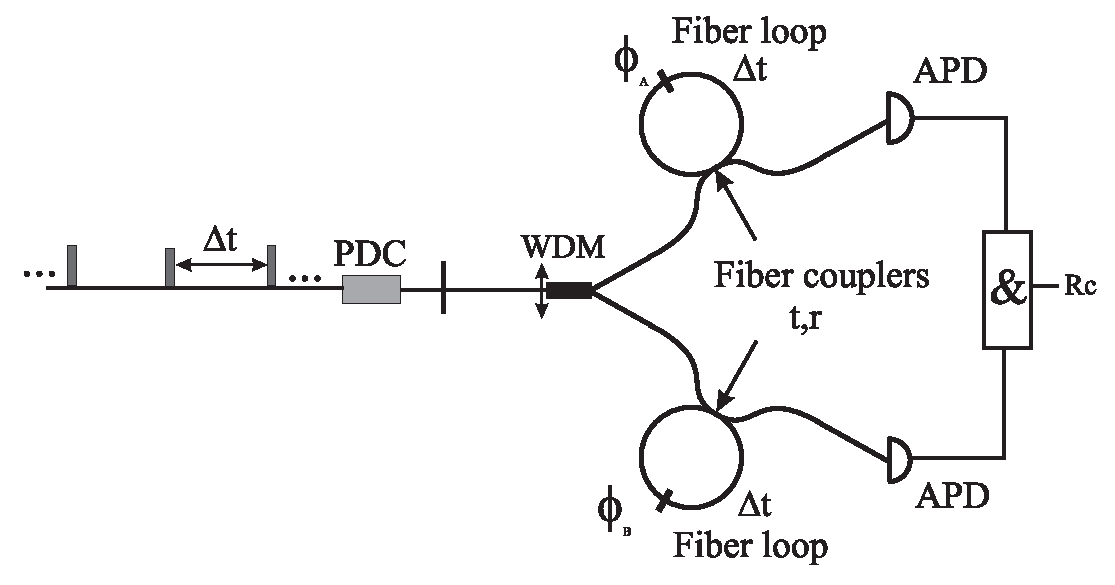
\epsfig{file=fig1.eps, width=8.2cm}} %100 percent
\vspace*{13pt}
\fcaption{\label{motion}figure caption goes here.}
\end{figure}

Figures are to be sequentially numbered in Arabic numerals. The
caption must be placed below the figure. Typeset in 8 pt Times
Roman with baselineskip of 10~pt. Use double spacing between a
caption and the text that follows immediately.

Previously published material must be accompanied by written
permission from the author and publisher.

\section{Tables}
\noindent
Tables should be inserted in the text as close to the point of
reference as possible. Some space should be left above and below
the table.

Tables should be numbered sequentially in the text in Arabic
numerals. Captions are to be centralized above the tables.
Typeset tables and captions in 8 pt Times Roman with
baselineskip of 10 pt.

\vspace*{4pt}   %only when needed
\begin{table}[hb]
\tcaption{Number of tests for WFF triple NA = 5, or NA = 8.}
\centerline{\footnotesize NP}
\centerline{\footnotesize\smalllineskip
\begin{tabular}{l c c c c c}\\
\hline
{} &{} &3 &4 &8 &10\\
\hline
{} &\phantom03 &1200 &2000 &\phantom02500 &\phantom03000\\
NC &\phantom05 &2000 &2200 &\phantom02700 &\phantom03400\\
{} &\phantom08 &2500 &2700 &16000 &22000\\
{} &10 &3000 &3400 &22000 &28000\\
\hline\\
\end{tabular}}
\end{table}

If tables need to extend over to a second page, the continuation
of the table should be preceded by a caption, e.g.~``({\it Table
2. Continued}).''

\section{References Cross-citation}
\noindent
References cross-cited in the text are to be numbered consecutively in
Arabic numerals, in the order of first appearance. They are to
be typed in brackets such as \cite{first}  and \cite{cal, niel, mar}.
%superscripts after punctuation marks,
%e.g.~``$\ldots$ in the statement.$^5$''.

\section{Sections Cross-citation}\label{sec:abc}
\noindent
Sections and subsctions can be cross-cited in the text by using the latex command
shown here. In Section~\ref{sec:abc}, we discuss ....
%\newpage

\section{Footnotes}
\noindent
Footnotes should be numbered sequentially in superscript
lowercase Roman letters.\fnm{a}\fnt{a}{Footnotes should be
typeset in 8 pt Times Roman at the bottom of the page.}

\nonumsection{Acknowledgements}
\noindent
We would thank ...

\nonumsection{References}
\noindent
References are to be listed in the order cited in the text.
For each cited work, include all the authors' names, year of the work, title,
place where the work appears.
Use the style shown in the following examples. For journal names,
use the standard abbreviations. Typeset references in 9 pt Times
Roman.

\begin{thebibliography}{000}
\bibitem{first}
P. Horodecki and R. Horodecki (2001), {\it Distillation and bound entanglement},
Quantum Inf. Comput., Vol.1, pp. 045-075.

\bibitem{cal}
R. Calderbank and P. Shor (1996), {\it Good quantum error
       correcting codes exist},
Phys. Rev. A, 54, pp. 1098-1106.

\bibitem{niel}
M.A. Nielsen and J. Kempe (2001), {\it Separable states are
more disordered globally than locally}, quant-ph/0105090.

\bibitem{mar}
A.W. Marshall and I. Olkin (1979), {\it Inequalities: theory of majorization and its applications},
Academic Press (New York).
\end{thebibliography}

\appendix

\noindent
Appendices should be used only when absolutely necessary. They
should come after the References. If there is more than one
appendix, number them alphabetically. Number displayed equations
occurring in the Appendix in this way, e.g.~(\ref{that}), (A.2),
etc.
\begin{equation}
\langle\hat{O}\rangle=\int\psi^*(x)O(x)\psi(x)d^3x~. 
\label{that}
\end{equation}

\end{document}
